\section{Methodology}
\subsection{Preliminary Analysis}
At an earlier stage of the project, we plan to build an octave piano with twelve notes including minor keys. At that stage, we analyzed the frequency spectrum of each note and found out it is possible to produce a majority feeling of sound with only four harmonics to a given note.
\par
After synthesizing all the keynotes from its harmonics using Matlab, we moved to circuit development. At this stage, we decided to stimulate only one note from the piano because the generation of notes is modularizable. For this purpose, we have chosen the C-wave which is in the middle of the spectrum.
\begin{figure}[h]
    \begin{subfigure}{.45\columnwidth}
        \centering
        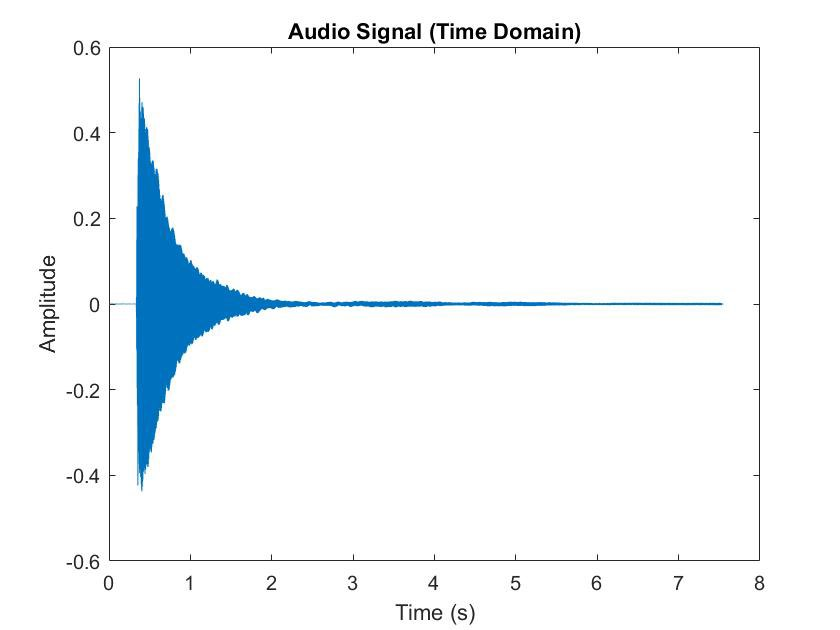
\includegraphics[width=.9\columnwidth]{c_wave}
    \end{subfigure}
    \begin{subfigure}{.45\columnwidth}
        \centering
        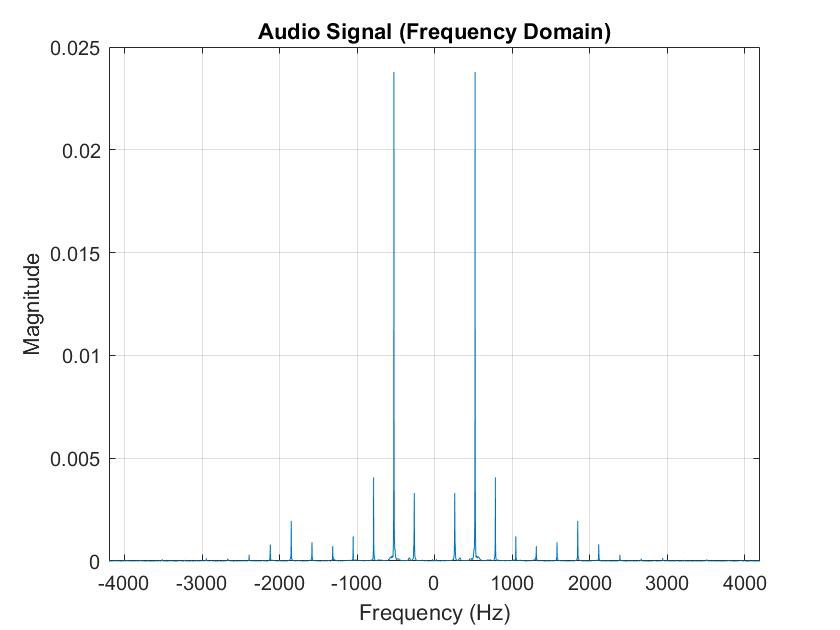
\includegraphics[width=.9\columnwidth]{spectrum_c}
    \end{subfigure}

\end{figure}
\subsection{Circuit Design}
The key components of the circuit are illustrated below in the block diagram. Before moving to the prototype all the circuits are simulated using NI Multism.Working simulation models of all the circuits can be found in the git-repository.
\begin{figure}[h]
    \begin{center}
        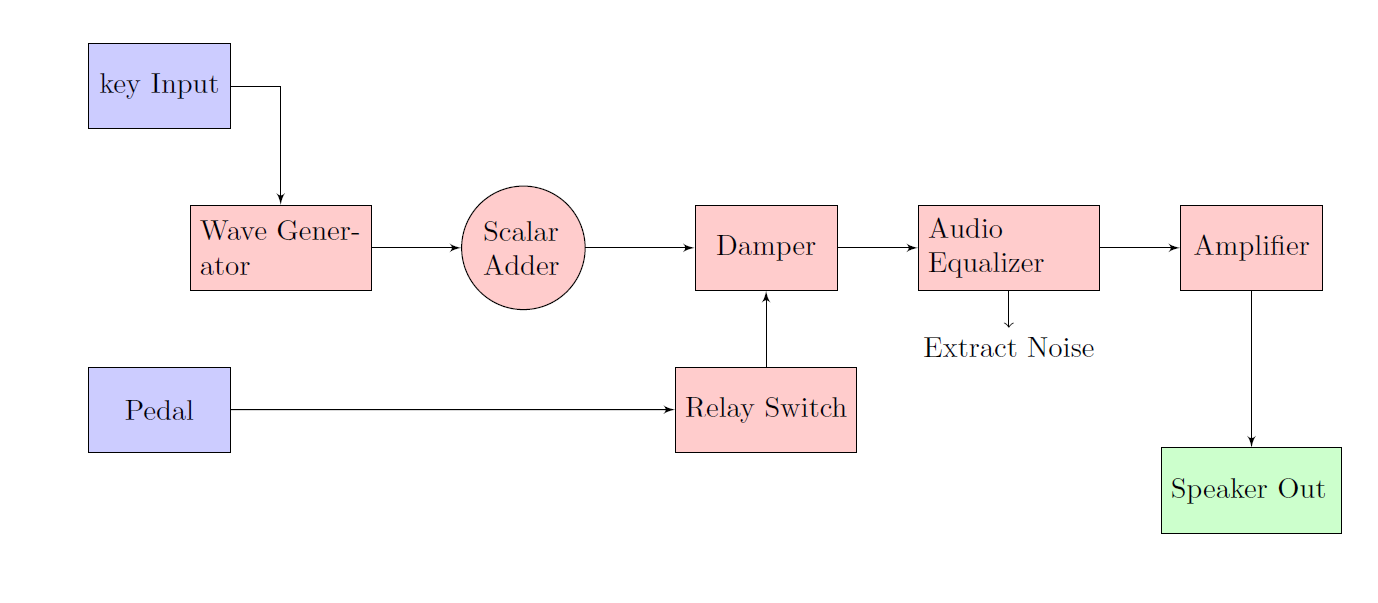
\includegraphics[width=\columnwidth]{flow}
        \caption*{Block Diagram of the Circuit}
    \end{center}
\end{figure}
\subsubsection{Wave Generator}
Square wave generation of half the frequency together with a bandpass active filter is considered in the first stage of the circuit development. Need for achieving a larger Q factor for the filter as the number of harmonics increases, lift the choice to not-feasible.
\par
Moving towards a stable solution brought the Wien bridge oscillator into play. These oscillators have the flexibility over frequency choice ($\frac{1}{2\pi RC}$) making them the most suitable option to be used with modularizable piano.
\subsubsection{Key and Pedal}
After a clear analysis of the waveform using Matlab, it is expected to achieve an exponential decay in the waveform once the oscillation is triggered. Looking at the discharging behavior of the capacitor initially it decided to engage a capacitor together with an analog multiplier to form an envelope around wave output.
\par
Due to the power inefficiency of the design and difficulty in finding good quality multipliers, the design moved to engage tuning of negative feedback of oscillator to achieve necessary output. This is further utilized to mimic the damping pedal of the piano by controlling the elongation of the signal-out of each oscillator.
\subsubsection{Scalar Adder}
Direct connection between outputs of oscillators even after scaling leads to interference in the signal generation stage of the oscillator. In contrast, using a scaling adder we can provide a low impedance output path while scaling the inputs as specified.
\subsubsection{Amplifier}
At earlier stages, the amplifier was implemented in class-A configuration. The requirement for lower output resistance of the bias path leads to high power dissipation in the signal-free state. This made such a model not practical without huge heatsinks at the cost of low power efficiency.
\begin{figure}[h]
    \begin{center}
        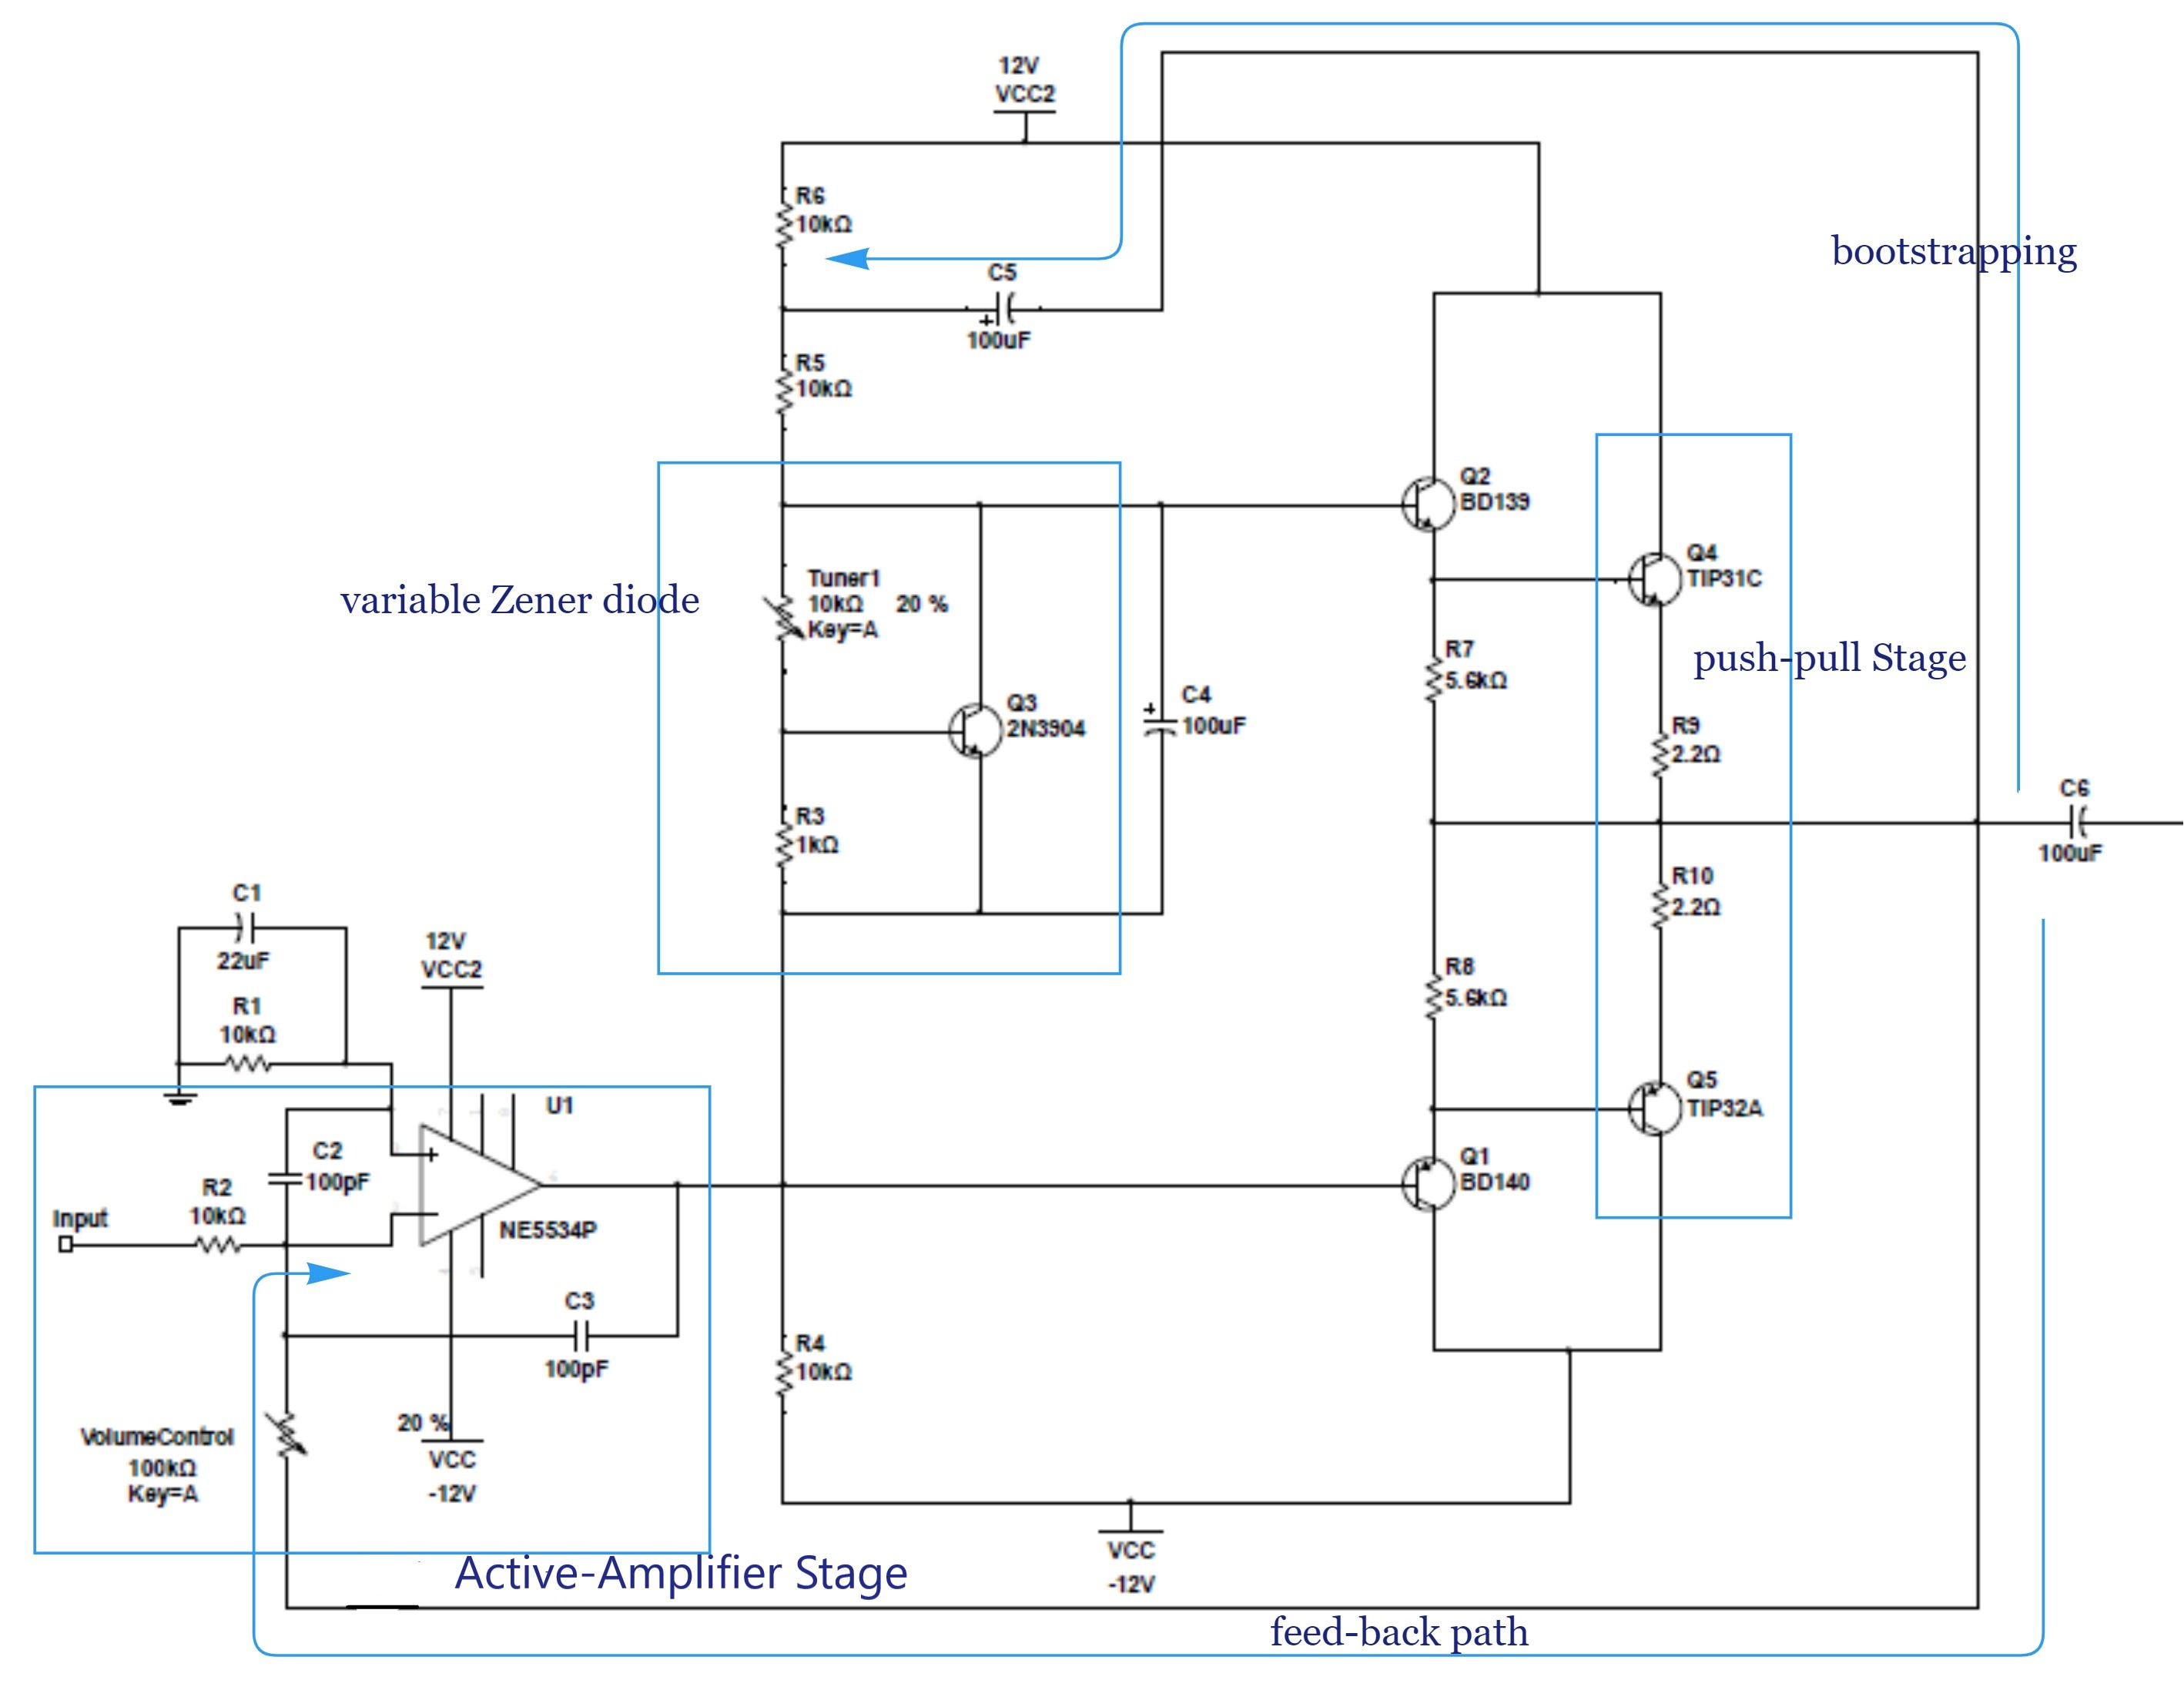
\includegraphics[width=\columnwidth]{amplifier_cd}
    \end{center}
\end{figure}
\\
\textbf{Active Amplifier Stage}: In the first part of the amplifier design an op-amp is used in the inverting configuration. The feedback path is connected to the end of the overall circuit to ensure enough current supply available in the output.\\
The op-amp NE5534 was chosen for the purpose according to its key characteristics such as high unity-gain bandwidth(10MHz), very low harmonic distortion,high common mode rejection ratio(100dB). The capacitance values of C2 and C3 are chosen to allow only higher frequencies ($>20kHz$) to pass through. These are utilized in a manner to remove high-frequency noises from the wave-form.
\\
\\
\textbf{Push-Pull Stage}: Considering the requirement of high power gain it is decided to engage Darlington pairs for this purpose. These components failed in the long run due to the inability of compensating for high power dissipation. Considering this, the design moved to engage two coupled BJTs to allow the choices for transistors to be used in the high current path. The similar pairs TIP31C and TIP32C were chosen after considering their high power compensation capability(around 40W).
\\
\\
\textbf{Bias}: Due to the requirement for a sudden supply of high current on the keypress, the signal gets noisy when we drive the speaker without any bias. In earlier stages, a few diodes are used to bias the circuit which failed to get rid of the noise. As the next step, we used Zener diodes that provide the capability to choose higher bias voltage. This results in the low efficiency of the circuit.
After considering all the methods it is decided to implement the variable Zener diode which has the flexibility over varying bias voltage in a wider range. This provides control over two extremities, effecieny and quality of the output.
\\
\\
\textbf{Bootstrapping}: The capacitor C5 gets charged to the pre-decided bias voltage.  By maintaining the circuit time constant very large ($t=R5\parallel R6\star C5>0.5S$) the overall bias voltage of the circuit is maintained at a constant value through-out the signal time.

\subsection{Prototype Design}
\begin{figure}[h]
    \begin{minipage}{.53\columnwidth}
        At earlier stages, a virtual prototype was developed using Multisim(see Appendix A), and many of the tests were carried out on this program itself. Afterward, the model is moved to the breadboard in a modular manner and the outputs at each stage were tested independently.
    \end{minipage}
    \begin{minipage}{.38\columnwidth}
        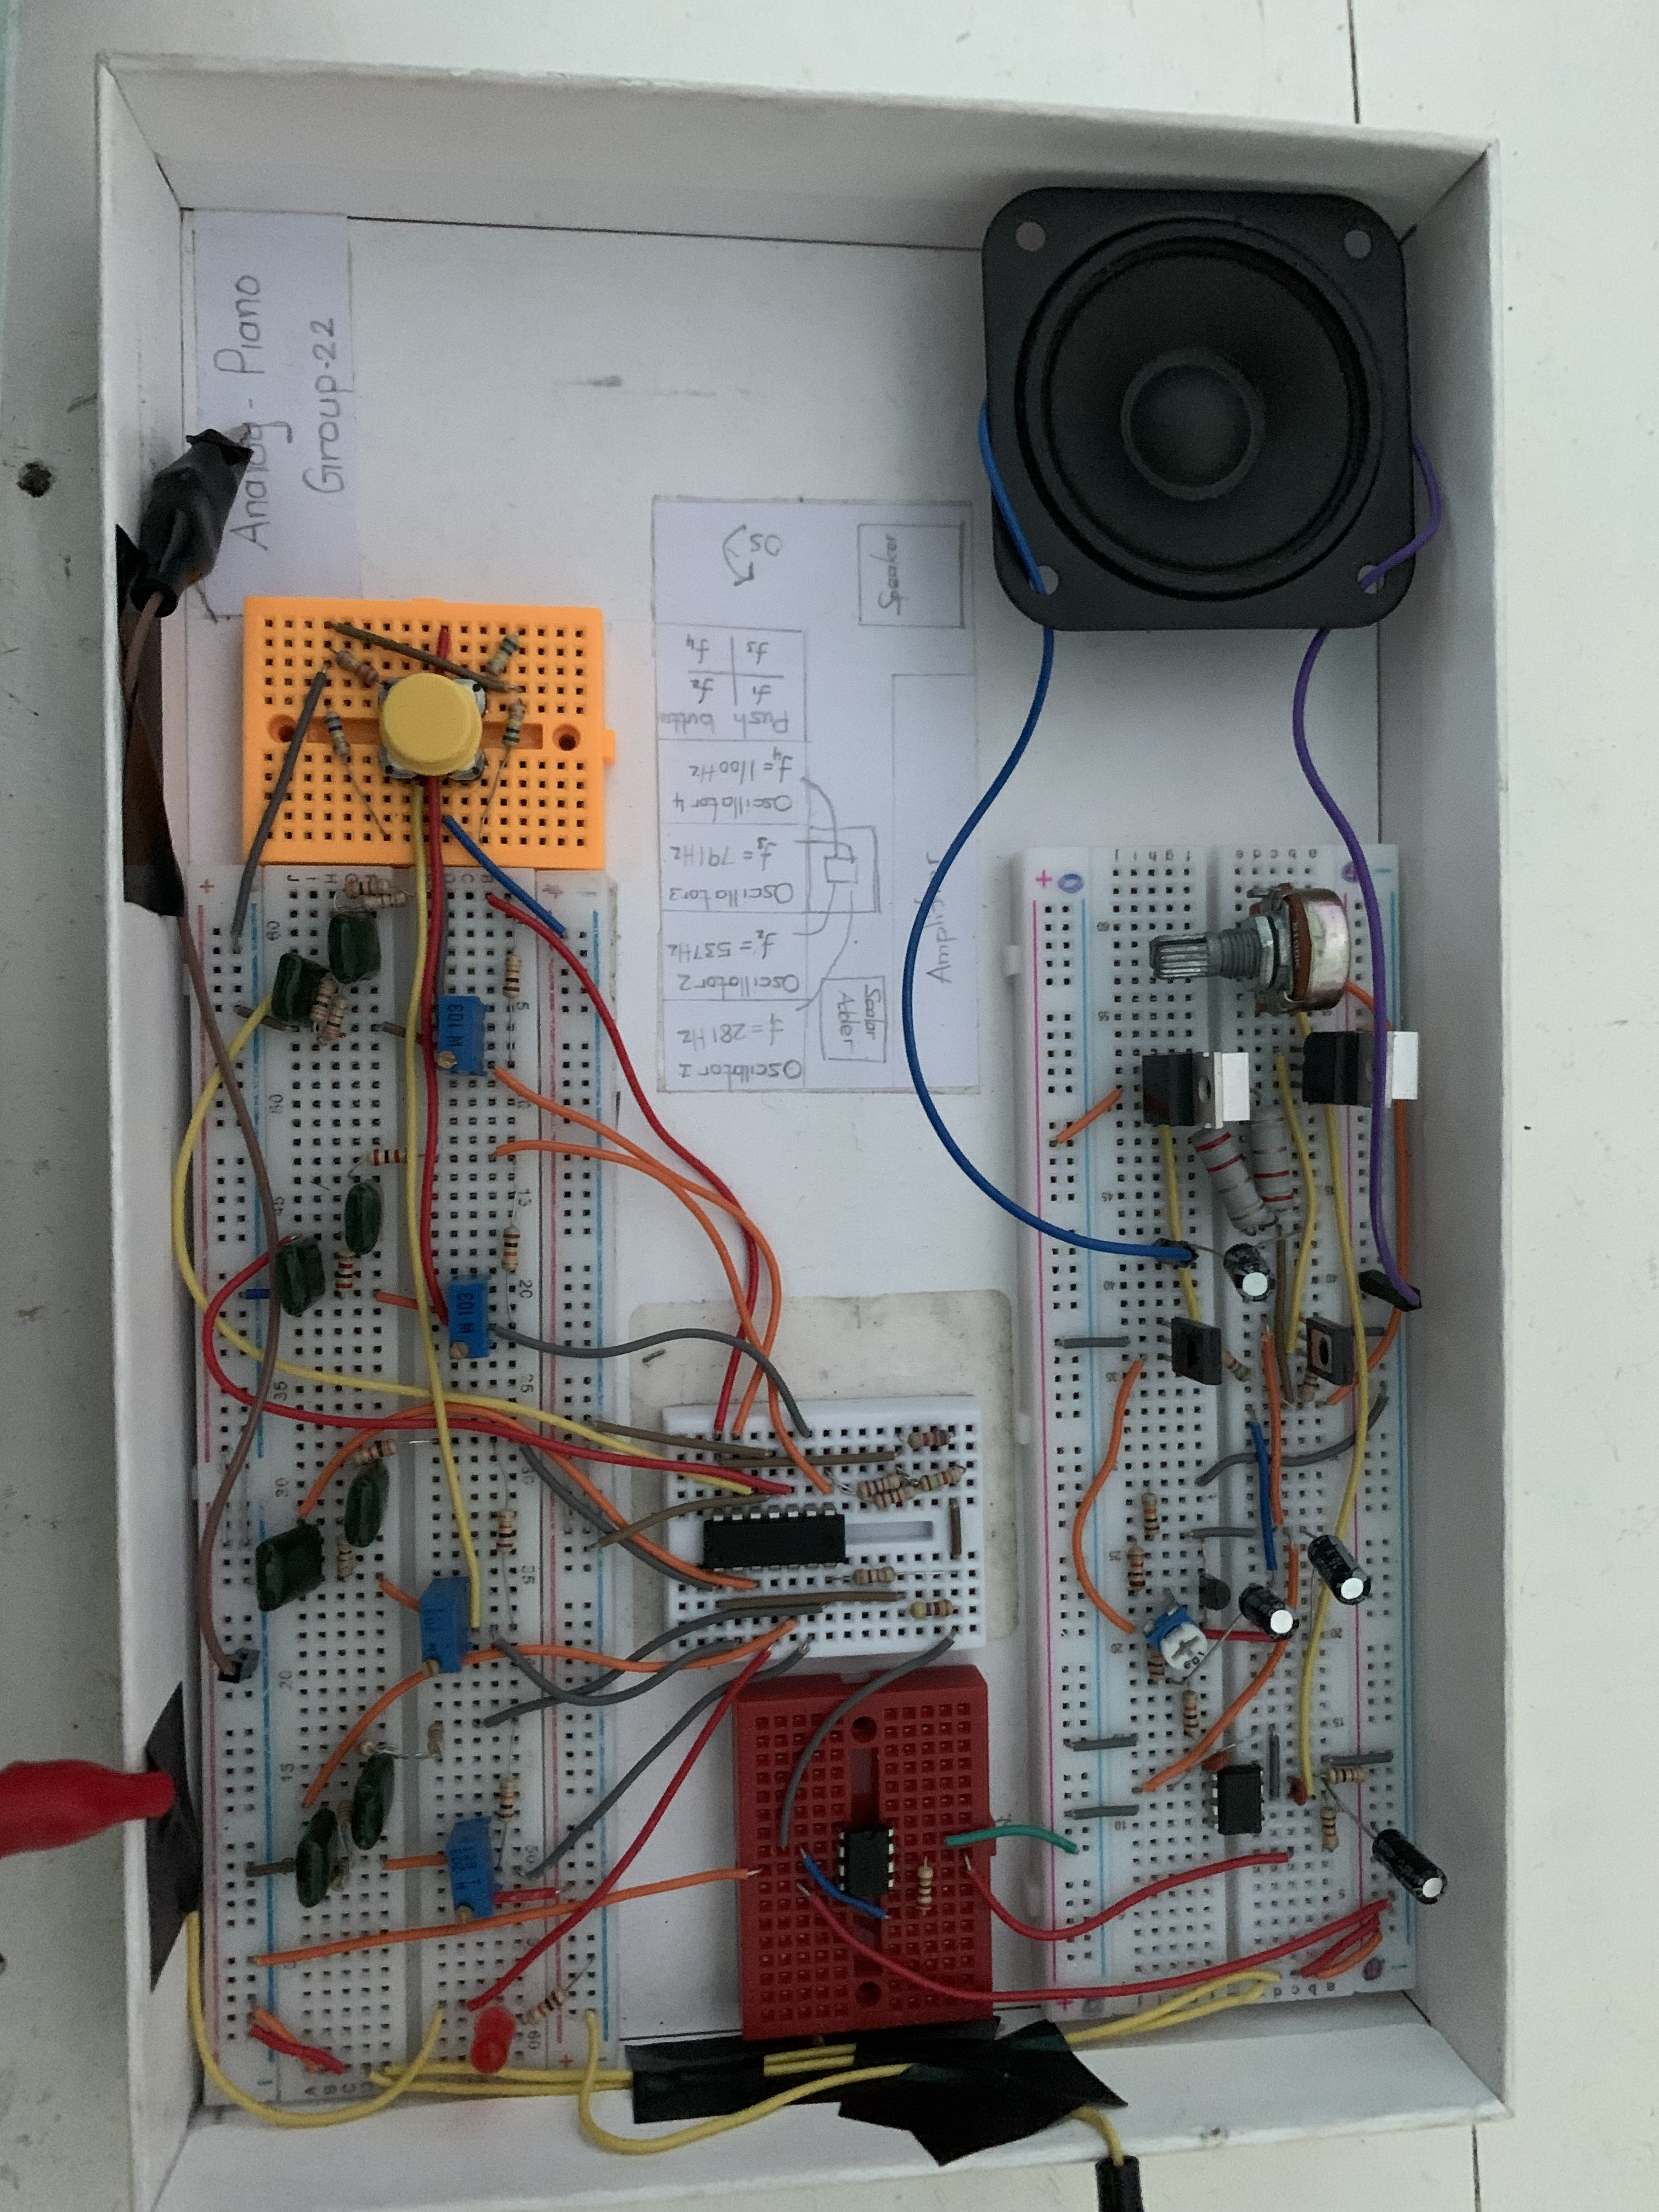
\includegraphics[width=.95\columnwidth]{breadboard}
    \end{minipage}
\end{figure}

As the final step of implementation, PCB for the physical prototype was designed using Altium (see Appendix B for layout). This was then screen printed and the relevant components soldered to the PCB. Finally, heatsinks were mounted accordingly to ensure safer operation.
\subsection{Components}
\subsubsection*{Wave Generator}
The resistance and capacitance values corresponding to the filter circuit of each frequency in the oscillator are indicated below in the table. The normalized content ratio and resistance used in the input path of the scalar adder are also appended together.
\begin{center}
    \begin{tabular}{|c|c|c|c|c|}
        \toprule
        f    & \multicolumn{2}{|c|}{Oscillator} & \multicolumn{2}{|c|}{Scaling}                         \\
        \cmidrule{2-5}
        (Hz) & R(k$\Omega$)                     & C(nF)                         & $\eta$ & R(k$\Omega$) \\
        \midrule
        281  & 5.67                             & \multirow{4}{*}{100}          & 0.1386 & 3.03         \\
        537  & 2.96                             &                               & 1      & 420          \\
        791  & 2.01                             &                               & 0.168  & 2.5          \\
        1087 & 1.44                             &                               & 0.051  & 8.33         \\
        \bottomrule
    \end{tabular}
\end{center}

Easily available 4-quad op-amp LM341 was chosen for oscillators. This allowed having a compact design in prototyping. UA751 op-amp is used in the scalar adder stage and 220ohm is used as feedback resistance to ensure the addition of all four waves sits in the supply range.
\subsubsection*{Amplifier}
The following list of elements is used in the amplifier stage to allow only the frequency in the audible range to pass through and to withstand high power dissipation.
\begin{enumerate}
    \item Capacitors :
          \begin{tabular}{l r}
              22$\mu$F  & 1 \\
              100$\mu$F & 1 \\
              100pF     & 2 \\
          \end{tabular}
    \item Resistors :
          \begin{tabular}{l r}
              10k$\Omega$  & 5 \\
              1k$\Omega$   & 1 \\
              5.6k$\Omega$ & 2 \\
          \end{tabular}
    \item Presets :
          \begin{tabular}{l r}
              10k$\Omega$  & 1 \\
              100k$\Omega$ & 1 \\
          \end{tabular}
    \item Power Resistors :
          \begin{tabular}{l r}
              2.2$\Omega$ & 2 \\
          \end{tabular}
    \item Transistors :
          \begin{tabular}{l r}
              2N3904        & 1 \\
              TIP31C,TIP32C & 1 \\
              BD139,BD140   & 1 \\
          \end{tabular}
    \item Op-Amp : NE5534P   1
\end{enumerate}